\begin{wrapfigure}{l}{0.1\textwidth}
                
\includegraphics[width=\linewidth]{images/ikony_pliki.png}
\end{wrapfigure}

Menadżer plików jest programem służącym do przeglądania zawartości katalogów. W Ubuntu menadźer plików nazywa się \textcolor{ubuntu_orange}{Nautilus} i jest odpowiednikiem programu \textcolor{ubuntu_orange}{Eksplorator Windows} z systemów Windows oraz \textcolor{ubuntu_orange}{Finder} z Mac OX X. Na pasku Launchera Nautilus domyślnie jest drugą dostępną ikoną. 

Program Pliki po uruchomieniu wyświetla zawartość katalogu domowego użytkownika, w którym to użytkownik przechowuje swoje osobiste pliki. Każdy użytkownik ma swój oddzielny katalog domowy, którego nazwa odpowiadania nazwie użytkownika. Po utworzeniu konta w katalogu domowym automatycznie utworzone są katalogi Dokumenty, Muzyka, Obrazy, Pobrane, Publiczny, Pulpit, Szablony, Wideo. Użytkownik nie jest ograniczony jedynie do tych katalogów i bez problemu w katalogu domowym może dodać więcej katalogów oraz plików.

\begin{center}
	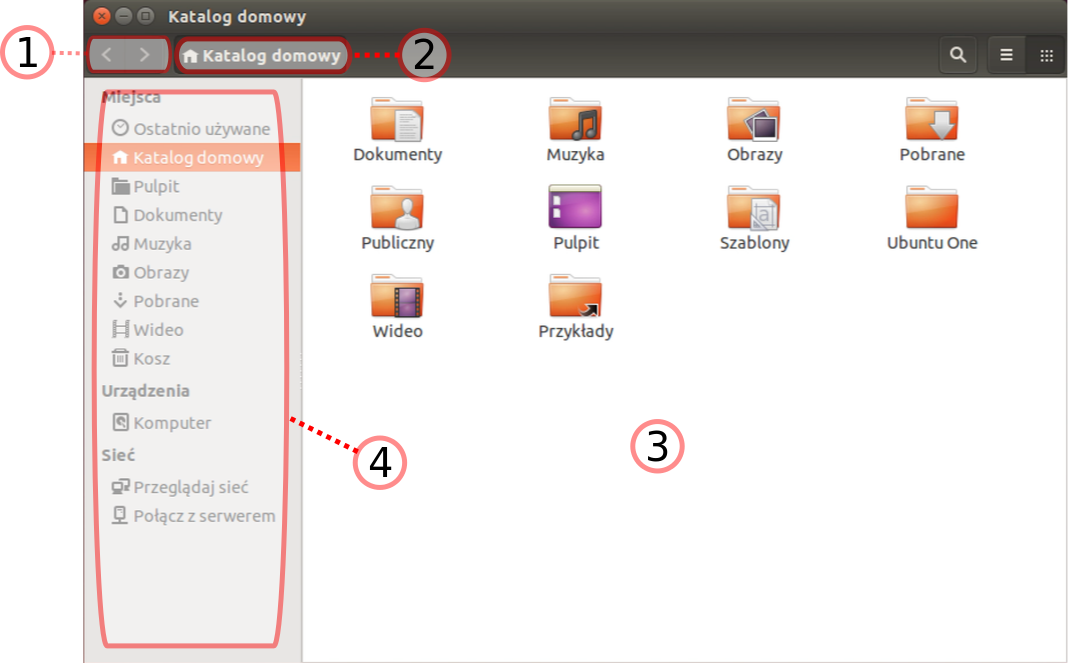
\includegraphics[width=\linewidth]{images/programy_nautilus.png}
\end{center}

W oknie menadżera plików widzimy:
\begin{enumerate}[label=\protect\circled{\arabic*}]
\item Przyciski \textcolor{ubuntu_orange}{Do tyłu} i \textcolor{ubuntu_orange}{Do przodu}.
\item Aktualne położenie.
\item Zawartośc aktualnego katalogu.
\item Pasek ze skrótami do najważniejszych miejsc.
\end{enumerate}

Menadżer plików w lewym panelu będzie też wyświetlał podłączone urządzenia (pendrive, karty SD, płyty włożone do czytników optycznych) oraz udziały sieciowe (inne podłączone komputery). Pozycja \textcolor{ubuntu_orange}{Komputer} przenosi do początku systemu plików (katalog /)

Do nawigacji w pasku narzędzi oraz lewym panelu wykorzystywane jest pojedyncze kliknięcie lewym przyciskiem myszy. W prawym panelu pliki oraz katalogi domyślnie otwieramy dwukrotnym szybkim przyciśnięciem lewego przycisku myszy. W przypadku otwarcia pliku, Ubuntu rozpozna typ pliku i automatycznie spróbuje przypisać odpowiednią dla danego pliku aplikację. Czasami, system może nie rozpoznać typu pliku lub może zajść potrzeba otwarcia pliku wykorzystując inny program. W takich wypadkach, po dwukrotnym kliknięciu na pliku system zapyta nas, który program z zainstalowanych w systemie chcemy wykorzystać. Możemy również nacisnąć prawym przyciskiem myszy na pliku i z menu kontekstowego wybrać Otwórz za pomocą i wybrać z listy dostępnych programów lub samemu wybrać inny.

Najważniejsze katalogi w folderze użytkownika:
\begin{itemize}
\item \textcolor{ubuntu_orange}{Pulpit} - wszystkie pliki i foldery umieszczone w tym katalogu zostaną wyświetlone na pulpicie.
\item \textcolor{ubuntu_orange}{Dokumenty} - katalog na dokumenty, pliki tekstowe, arkusze kalkulacyjne itp.
\item \textcolor{ubuntu_orange}{Muzyka} - katalog z plikami muzycznymi. Odtwarzacze muzyki będą szukać plików do odtwarzania najpierw w tym folderze.
\item \textcolor{ubuntu_orange}{Wideo} - katalog z plikami wideo.
\item \textcolor{ubuntu_orange}{Obrazy} - katalog z fotografiami.
\item \textcolor{ubuntu_orange}{Pobrane} - katalog na pliki pobrane z internetu. przeglądaki internetowe domyślnie będą zapisywać pobrane pliki w tym katalogu.
\end{itemize}

\subsubsection{Tworzenie nowych katalogów}
Tworzenie nowych katalogów niczym nieróżni się się od metod, które dostępne są w innych systemach. Zwyczajnie wystarczy nacisnąć prawym przyciskiem myszy na wolnej przestrzeni w oknie programu (ta metoda również zadziała na naszym pulpicie) i z menu kontekstowego wybrać opcję \textcolor{ubuntu_orange}{Nowy katalog}. Można również wykorzystać w tym celu panel menu i wybrać \menu{Plik>{Nowy katalog}}. Można również wykorzystać skrót klawiaturowy \keys{Shift + CTRL + n}.

\subsubsection{Ukryte pliki i katalogi}
Ubuntu, jak każdy inny Linux, umożliwia tworzenie ukrytych plików oraz katalogów. Aby ukryć plik lub katalog, wystarczy w jego nazwie na samym początku wstawić znak kropki (.). Gdy chcemy uzyskać dostęp do ukrytych plików lub katalogów, należy z panelu menu wybrać \menu{Widok>Wyświetlanie ukrytych plików} lub skorzystać ze skróty klawiaturowego \keys{CTRL + h}.

UWAGA: Wyświetlenie ukrytych plików w katalogu domowym użytkownika wyświetli wiele dodatkowych plików oraz katalogów, które w większości przypadków przechowują ustawienia dla wielu programów użytkownika, wyglądu konta użytkownika oraz zachowań na koncie użytkownika. Niewłaściwe obchodzenie się z tymi plikami, może mieć negatywne skutki. Zaleca się zatem dodatkową ostrożność.

\subsubsection{Kopiowanie i przenoszenie plików oraz katalogów}
Ubuntu, jak każdy inny system również umożliwia kopiowanie i przenoszenie plików oraz katalogów z jednego miejsca do innego. Aby plik lub katalog skopiować lub przenieść z jednego miejsca do innego, trzeba go najpierw zaznaczyć, a następnie nacisnąć na obiekcie prawym przyciskiem myszy i wybrać z menu kontekstowego skopiuj (w przypadku, gdy chcemy go utworzyć kopię) lub wytnij (w przypadku, gdy plik chcemy przenieść), a następnie przechodzimy do katalogu, w którym plik chcemy umieścić i w wolnym miejscu naciskamy prawym przyciskiem myszy i wybieramy wklej. Te same opcje dostępne są z panelu menu i znajdują się one w menu Edycji.

W menu kontekstowym pod prawym przyciskiem myszy mamy również opcję \textcolor{ubuntu_orange}{Skopiuj do \ldots} oraz \textcolor{ubuntu_orange}{Przenieś do \ldots} po wybraniu których, będziemy mieli możliwość wybrania folderu, w którym chcemy umieścić nasz plik lub katalog.
Do powyższych czynności, możemy również wykorzystać skróty klawiaturowe. Aby skopiować zaznaczony obiekt, należy użyć skrót \keys{CTRL + c}, aby go przenieść \keys{CTRL + x}, aby wkleić obiekt w nowym miejscu, należy użyć skrót \keys{CTRL + v}.

Aby zaznaczyć wiele obiektów naraz, należy na wolnym miejscu w oknie nacisnąć i przytrzymać lewy przycisk myszy po czym zaznaczyć wybrane elementy. Gdy pliki znajdują się koło siebie, można wykorzystać przycisk \keys{Shift} i przytrzymując go należy najpierw pojedynczym kliknięciem lewym przyciskiem myszy zaznaczyć pierwszy obiekt, a następnie ciągle przytrzymując przycisk \keys{Shift} kliknąć na ostatni obiekt. Gdy obiekty, które chcemy zaznaczyć, przedzielone są innymi obiektami, wówczas pomocny może się okazać przycisk \keys{CTRL}, którego przytrzymanie również umożliwia zaznaczenie wielu elementów, tyle że niekoniecznie muszą one być koło siebie.

\subsubsection{Wyszukiwanie plików w programie Pliki.}
\begin{center}
	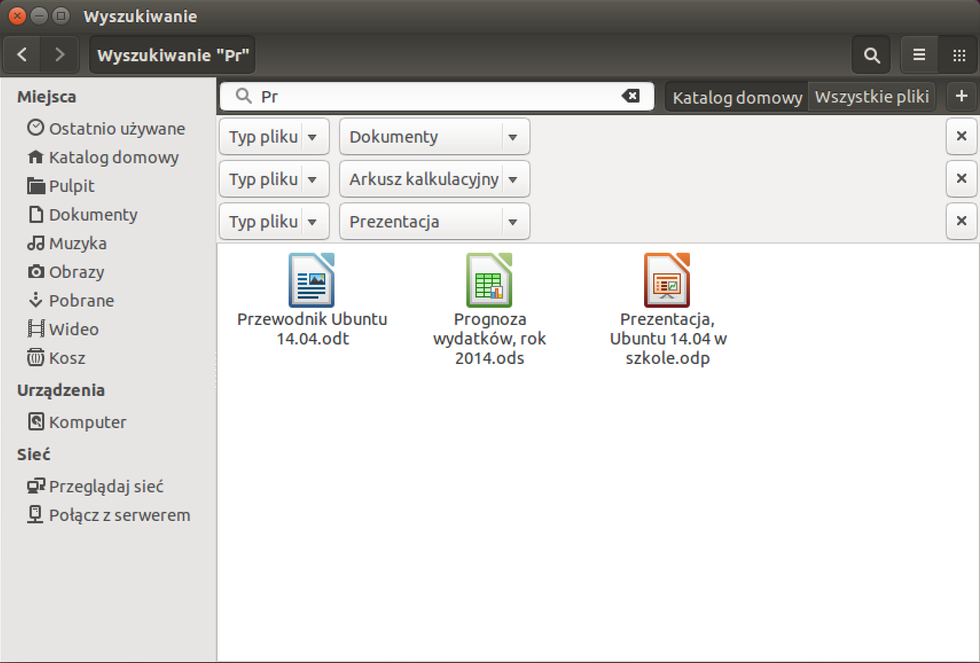
\includegraphics[width=\linewidth]{images/programy_nautilus2.png}
\end{center}

To, że Dash jest potężnym narzędziem i że pozwala wyszukiwać pliki już wiemy. Ale pliki i katalogi również możemy wyszukiwać wykorzystując okno programu Pliki. Jak już wcześniej wspomnieliśmy, w oknie programu na pasku narzędzi znajduje się przycisk wyszukiwania (ikona szkła powiększającego). Po naciśnięciu na przycisku wyszukiwania pojawi się pasek, w którym to podajemy frazę (nazwę pliku lub katalogu) do wyszukania. Rezultaty wyszukiwania, podobnie jak to jest w Dashu, możemy filtrować. Możemy określić, czy wyszukiwanie ma się odbywać z obrębie naszego katalogu domowego lub w całym systemie. Możemy również dodać dodatkowe kryteria wyszukiwania określając, jakiego typu pliki szukamy.
\subsubsection{Używanie wielu okien lub wielu kart w programie Pliki}
W przypadku kopiowania lub przenoszenia plików pomocne może być otwarcie wielu okien lub kart. Nowe okno programu pliki można otworzyć na wiele sposób:
\begin{itemize}
\item wykorzystując panel menu i przycisk \menu{{Plik}>{Nowe okno}}.
\item naciskając prawym przyciskiem myszy na ikonie programu Pliki na pasku Launchera i wybierając z menu kontekstowego \textcolor{ubuntu_orange}{Otwórz nowe okno}.
\item wykorzystując skrót klawiaturowy \keys{CTRL + n}.
\end{itemize}
Program Pliki umożliwia również pracę z kartami, które również można otworzyć na wiele sposobów:
\begin{itemize}
\item wykorzystując panel menu i przycisk \menu{Plik >{Nowa karta}}.
\item naciskając prawym przyciskiem myszy na dowolny folder w oknie programu i wybierając z menu kontekstowego \textcolor{ubuntu_orange}{Otwórz w nowej karcie}.
\item wykorzystując skrót klawiaturowy \keys{CTRL + t}.
\end{itemize}

\clearpage